\documentclass[11pt,a4paper]{article}
\usepackage[margin=24mm]{geometry}
\usepackage[utf8]{inputenc}
\usepackage{tikz}
\usetikzlibrary{positioning}
\title{Price quotes as model elements: unit prices derived, not typed}
\date{Created 2026-10-07 20:14 CEST}
\begin{document}
\maketitle
\paragraph{Scope and estimate.} The halfarm procurement lines carry a typed net unit price; where
the shop showed a gross price, a pack price or several components, the arithmetic was done by hand
and only a note remains. User decision 2026-10-07 20:11: prices must come from the model, so that
every table is a view of it. ETA 2--3 hours. No benchmark.
\paragraph{Semantics.} \texttt{data/sysml/meta\_sysml\_structure.hymeko} gains element kinds
\texttt{price\_quote} (what the source shows: \texttt{amount}, \texttt{currency} $\to$ currency,
\texttt{vat\_included} -- the VAT rate contained in \texttt{amount}, 0 when the shown price is net --,
\texttt{pack} -- units the amount buys --, \texttt{source}, \texttt{date}, \texttt{quote\_text}) and
\texttt{currency} (\texttt{rate}: home-currency units per unit), and the edge \texttt{priced\_by}
(+ price\_quote, $-$ product $|$ product\_candidate; field \texttt{per\_unit}: packs per item
unit). Net home-currency unit price $= \sum \texttt{per\_unit}\cdot\texttt{amount}/(1+\texttt{vat\_included})/
\texttt{pack}\cdot\texttt{rate}$. An item priced by quotes carries no typed price.
\paragraph{Ownership.} Transformation: the vocabulary additions, the structure witness and one test;
no engine change. Consumer: quotes and currencies in the model; one pricing module used by every
view (workbook with a sources sheet, requirement check, decision evaluation, model tests).
\paragraph{Tests.} Witness: quote, currency and \texttt{priced\_by} resolve with fields and roles.
Consumer: the derived prices reproduce today's typed ones where both exist (difference only from the
recorded VAT and pack); model tests -- an item has quotes or a typed price, never both; every quote has
a source and a date; typed prices are listed as not yet traceable. Counter-tests: a removed quote, a
changed VAT rate, a doubled price source.
\paragraph{Budget and risks.} Linear in quotes (about 60). Risk: VAT status not printed by a shop --
recorded as \texttt{vat\_included 0} with the quote text, and named in the report.
\paragraph{State and rollback.} \texttt{feat/material-lobes}, uncommitted; other workers' files
untouched; no git writes from the sandbox. Rollback: remove the three vocabulary lines and the test.
\begin{center}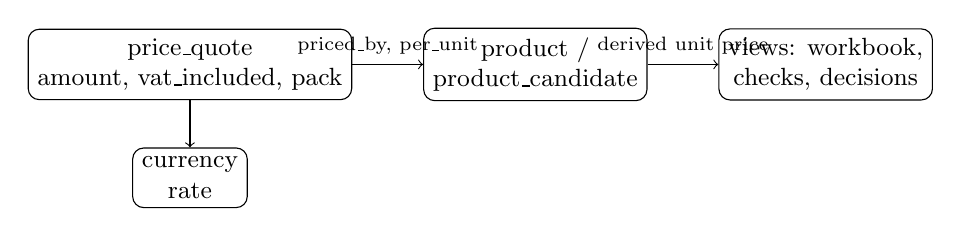
\begin{tikzpicture}[node distance=6mm and 9mm, every node/.style={draw, rounded corners, font=\small, align=center}]
\node (q) {price\_quote\\amount, vat\_included, pack};
\node (c) [below=of q] {currency\\rate};
\node (p) [right=of q] {product /\\product\_candidate};
\node (v) [right=of p] {views: workbook,\\checks, decisions};
\draw[->] (q) -- node[draw=none, above, font=\scriptsize]{priced\_by, per\_unit} (p);
\draw[->] (q) -- (c);
\draw[->] (p) -- node[draw=none, above, font=\scriptsize]{derived unit price} (v);
\end{tikzpicture}
\end{center}
\end{document}
